\chapter{CONCEPÇÃO E ENGENHARIA DO SISTEMA}
\label{chapter-4}
\section{Evolução da proposta e partes interessadas}
\label{section-4-1}
A concepção inicial pretendia oferecer apoio à contagem de prazos em diferentes ramos e ambientes. A revisão identificou que calendário, comunicação e exceções impediam tratar o objetivo amplo como uma única fórmula. A primeira decisão foi reduzir o escopo de implementação sem apagar o objetivo original. O backlog conserva expansões, enquanto cada perfil entregue declara suas condições.

As partes interessadas consideradas são a autora, a orientação, a banca, a pessoa que realiza a simulação e o responsável técnico pela instalação. Um profissional de Direito é necessário à revisão jurídica futura, mas sua aprovação não consta como concluída. O usuário anônimo pode calcular e consultar fontes; o autenticado pode manter o próprio histórico e solicitar lembretes. Administração normativa e trabalho em equipe não são papéis funcionais implementados.

\section{Escopo funcional e requisitos}
\label{section-4-2}
O quadro a seguir sintetiza o contrato efetivamente implementado. Os identificadores RF e RNF mantêm relação com docs/requirements.md; os limites dos perfis e os contratos posteriores complementam o documento histórico da primeira fatia.

\begin{quadro}[H]\centering
\caption{Requisitos funcionais do recorte entregue}
\label{quadro-1}
\begin{singlespace}\fontsize{10}{12}\selectfont
\begin{tabularx}{\linewidth}{|>{\raggedright\arraybackslash}X|>{\raggedright\arraybackslash}X|}
\hline
\textbf{ID} & \textbf{Comportamento verificável} \\
\hline
RF01 & Distinguir disponibilização e publicação no diário; identificar a data solicitada. AR e mandado permanecem fora do recorte. \\
\hline
RF02 & Aplicar a contagem do perfil selecionado, com marco excluído e primeiro dia computado separados. \\
\hline
RF03 & Selecionar calendário por tribunal, município e versão, conservando fontes dos eventos. \\
\hline
RF04 & Exibir marcos, trilha diária, motivo das decisões e vencimento quando determinável. \\
\hline
RF05 & Produzir estado incompleto e vencimento nulo quando faltar cobertura ou enquadramento. \\
\hline
RF06 & Exportar JSON e imprimir a memória com versões, avisos e fontes. \\
\hline
RF07 & Autenticar, salvar, listar e excluir somente cálculos da própria conta. \\
\hline
RF08 & Consultar calendários e fontes; não oferecer administração normativa remota. \\
\hline
RF09 & Agendar e cancelar lembrete opcional, com consentimento, fuso e situação de envio explícitos. \\
\hline
\end{tabularx}\end{singlespace}
\par\smallskip{\fontsize{10}{12}\selectfont Fonte: elaboração com base nos registros do projeto (2026).}
\end{quadro}
\begin{quadro}[H]\centering
\caption{Requisitos de qualidade e sua expressão no projeto}
\label{quadro-2}
\begin{singlespace}\fontsize{10}{12}\selectfont
\begin{tabularx}{\linewidth}{|>{\raggedright\arraybackslash}X|>{\raggedright\arraybackslash}X|}
\hline
\textbf{ID} & \textbf{Decisão e critério} \\
\hline
RNF01 & Motor determinístico, independente de rede, banco, React e relógio do sistema. \\
\hline
RNF02 & Datas civis em ISO/PlainDate; instantes de envio com fuso explícito de São Paulo. \\
\hline
RNF03 & Interface responsiva em pt-BR, erros associados, teclado e foco visível; WCAG AA como meta. \\
\hline
RNF04 & Validação e identidade no servidor, RLS, segredos fora do navegador e minimização de dados. \\
\hline
RNF05 & Versões e snapshots preservados; recomputação separada do original. \\
\hline
RNF06 & Tipos, lint, formatação, testes, build e migrations verificáveis por execução. \\
\hline
RNF07 & Hospedagem em Vercel e serviços Supabase integrados por ambiente. \\
\hline
\end{tabularx}\end{singlespace}
\par\smallskip{\fontsize{10}{12}\selectfont Fonte: elaboração com base nos registros do projeto (2026).}
\end{quadro}
As regras transversais exigem fonte primária e estado de revisão, recusam incompatibilidade territorial e temporal e preservam a indicação de demonstração. Calendário ausente não é substituído pelo de outra comarca. Contexto desconhecido não é convertido em ordinário. O servidor não recebe do navegador um calendário livre nem confia em um vencimento informado pelo cliente para salvar o histórico.

\section{Casos de uso e fluxo principal}
\label{section-4-3}
O fluxo público compreende selecionar perfil e localidade, identificar a comunicação, informar data e duração, calcular e examinar a memória. O fluxo privado acrescenta entrar, salvar, consultar, exportar ou excluir. O lembrete nasce de um cálculo salvo elegível e exige escolha expressa. Os casos de uso detalhados no Apêndice A registram precondições e alternativas, evitando descrever somente o caminho de sucesso.

\begin{figure}[H]\centering
\caption{Contexto e recursos disponíveis ao usuário}
\label{figure-1}
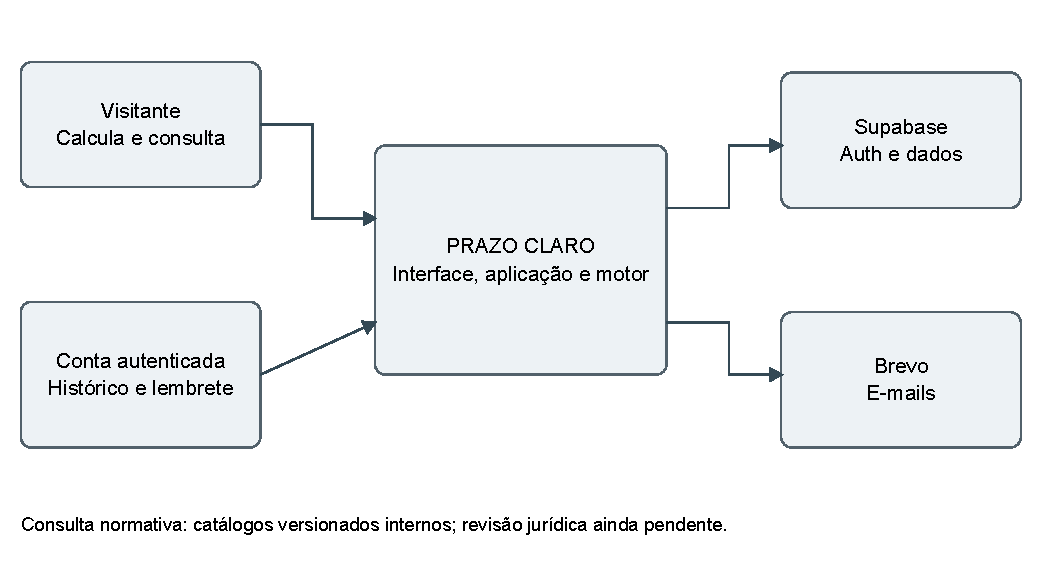
\includegraphics[width=\linewidth,height=.49\textheight,keepaspectratio]{figuras/contexto.pdf}
\par\smallskip{\fontsize{10}{12}\selectfont Fonte: elaboração para este relatório a partir do código e da documentação do Prazo Claro (2026).}
\end{figure}
As fronteiras externas da figura são reais: Supabase participa da identidade e dos dados, e Brevo participa das mensagens. A contagem pública não exige autenticação nem consulta remota durante a execução do motor. A indisponibilidade da configuração de conta é exibida sem apresentar uma sessão fictícia.

\section{Modelo de domínio}
\label{section-4-4}
O vocabulário distingue regime, perfil, suporte dos autos, meio de comunicação, evento, publicação, primeiro dia computado, fim nominal e vencimento. Uma regra versionada define o método dentro de um âmbito. O calendário versionado contém eventos e fontes. A entrada referencia as condições de seleção, e o resultado conserva trilha e cópias dos dados utilizados. Essas entidades lógicas não correspondem necessariamente a tabelas separadas.

\begin{figure}[H]\centering
\caption{Modelo conceitual de cálculo e memória}
\label{figure-2}
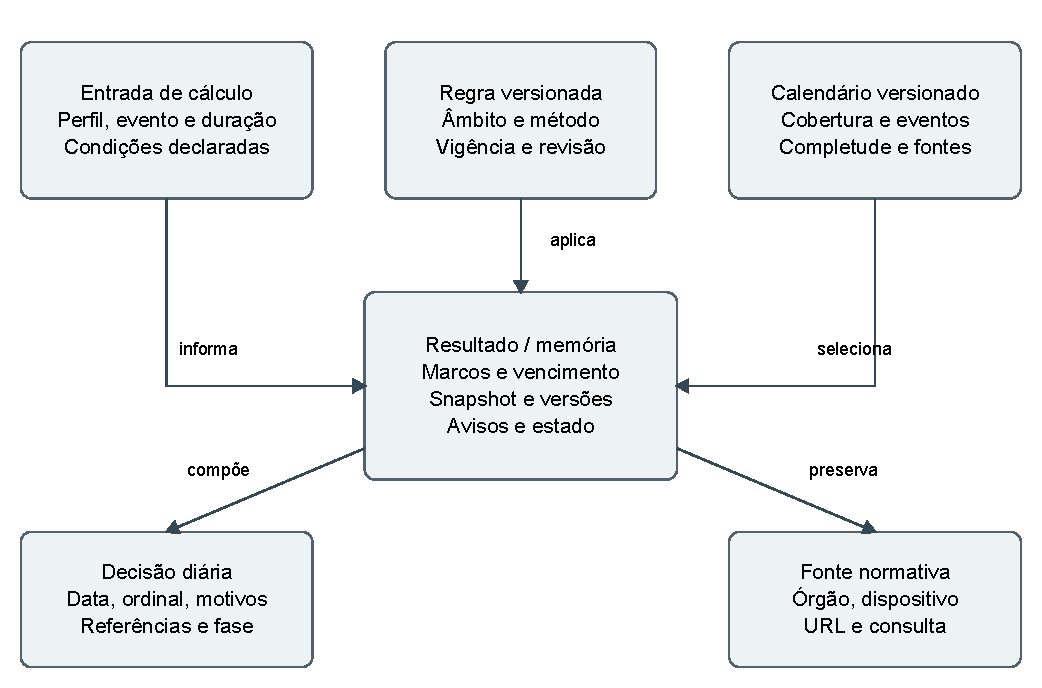
\includegraphics[width=\linewidth,height=.49\textheight,keepaspectratio]{figuras/dominio.pdf}
\par\smallskip{\fontsize{10}{12}\selectfont Fonte: elaboração para este relatório a partir do código e da documentação do Prazo Claro (2026).}
\end{figure}
A trilha é composta por decisões datadas: a data pode ser contada ou excluída, recebe ordinal quando consome unidade e conserva motivos e referências. O perfil criminal pode acrescentar uma fase de prorrogação sem consumir novas unidades. A memória mantém ainda pendências e estado de revisão, para que a exportação não transforme uma estimativa demonstrativa em resultado aprovado.

\section{Arquitetura e decisões}
\label{section-4-5}
A aplicação adota monólito modular. A apresentação reúne páginas e componentes React; a camada de aplicação valida contratos e seleciona dados; o domínio executa a contagem; adaptadores integram Supabase, e-mail e infraestrutura. Os catálogos normativos ativos são arquivos TypeScript versionados. As tabelas de catálogos do banco existem no schema, mas não constituem uma administração remota completa nem substituem a seleção utilizada pelo motor.

\begin{figure}[H]\centering
\caption{Camadas e dependências da implementação}
\label{figure-3}
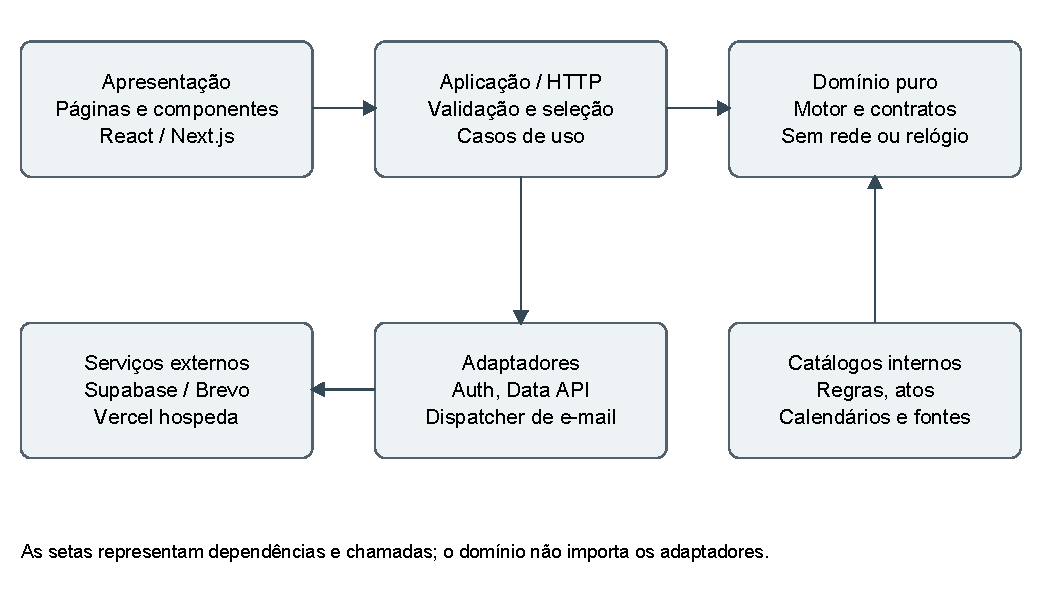
\includegraphics[width=\linewidth,height=.49\textheight,keepaspectratio]{figuras/arquitetura.pdf}
\par\smallskip{\fontsize{10}{12}\selectfont Fonte: elaboração para este relatório a partir do código e da documentação do Prazo Claro (2026).}
\end{figure}
Os ADRs registram seis decisões: motor independente e versões preservadas; Data API sem ORM inicial; histórico individual antes de organizações; novos perfis sem alterar o motor civil congelado; fila com tratamento de envio incerto; e agendamento com assinatura descartável. Não foram criados serviços NestJS ou um monorepo apenas para corresponder à proposta inicial. Uma separação futura depende de necessidade operacional demonstrada.

\section{Modelo físico e persistência}
\label{section-4-6}
O banco possui cinco tabelas públicas da aplicação: legal\_sources, legal\_rule\_versions, calendar\_versions, deadline\_calculations e deadline\_reminders. O schema reminder\_private contém configuração e invocações do agendador e funções internas. auth.users é gerenciada pelo Supabase Auth. Não existem tabelas públicas de organizações, membros, processos ou perfis administrativos neste recorte.

\begin{figure}[H]\centering
\caption{Relações físicas essenciais do banco}
\label{figure-4}
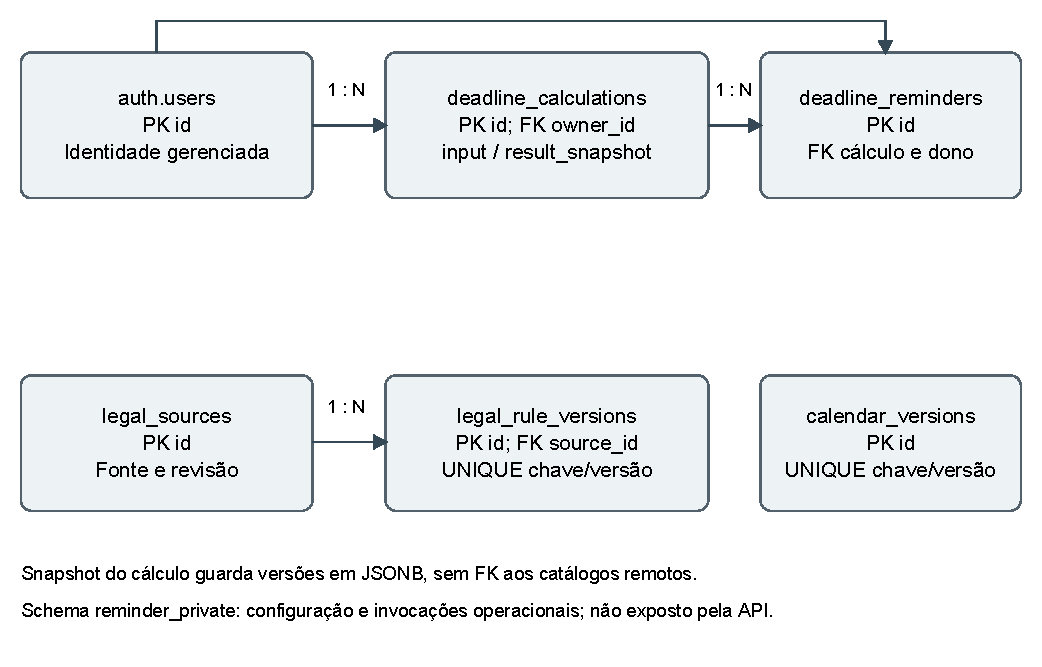
\includegraphics[width=\linewidth,height=.49\textheight,keepaspectratio]{figuras/dados.pdf}
\par\smallskip{\fontsize{10}{12}\selectfont Fonte: elaboração para este relatório a partir do código e da documentação do Prazo Claro (2026).}
\end{figure}
deadline\_calculations mantém proprietário, entrada e resultado em JSONB. O vínculo com versões normativas é preservado no snapshot; não existe uma chave estrangeira do cálculo para cada catálogo remoto. deadline\_reminders referencia cálculo e proprietário, com exclusão em cascata. Assim, apagar o cálculo remove o lembrete correspondente: essa consequência precisa ser compreendida antes de um ensaio de entrega.

Quatro migrations descrevem a evolução: 20261020001602 cria histórico e catálogos; 20261023172741 cria lembretes; 20261023184137 separa os modos de entrega; 20261023192044 instala o agendador. O dicionário do Apêndice B explicita campos e restrições. Atualizações usam migrations pendentes; reset de banco não é procedimento de manutenção de dados reais.

\section{Interface e experiência de uso}
\label{section-4-7}
O sistema utiliza um design system documentado, tipografia e espaçamento consistentes, campos rotulados e mensagens próximas à ação. A troca de perfil redefine escolhas incompatíveis. O ato opcional apresenta duração somente para leitura e exige confirmação específica; a quantidade manual permanece disponível. O resultado organiza data estimada, marcos, avisos, trilha e fontes, em vez de ocultar o contexto em uma nota genérica.

No histórico, o filtro por regime antecede a paginação no servidor. A busca textual é identificada como restrita à página atual. A situação futuro, hoje, passado ou indeterminado compara o vencimento original com a data de referência da aplicação, sem alterar o snapshot e sem afirmar cumprimento do ato. Estados vazios, carregamento, falha e exclusão possuem mensagens próprias.

Após cadastro aceito, uma página específica orienta a confirmar o e-mail no mesmo navegador, verificar spam e retornar ao acesso. Sua mensagem neutra evita revelar a existência de uma conta. A melhoria respondeu a um relato real: o e-mail chegava, mas a orientação permanecia no formulário. O contrato de confirmação e a proteção da sessão foram preservados.

\section{Segurança e tratamento de dados}
\label{section-4-8}
A identidade usada no servidor é obtida por verificação do usuário, e não por um ID confiado ao corpo da requisição. Políticas RLS restringem o histórico e a leitura de lembretes ao proprietário. Mutação privada confere origem e valida JSON. Chaves privilegiadas são exclusivas de código de servidor; a chave publicável e a existência de um botão oculto não substituem autorização.

Os fluxos de cadastro e recuperação apresentam mensagens genéricas. O callback troca código por sessão e restringe destinos. O fluxo de convite trata o retorno e permite definir senha; tokens e links de autenticação não integram logs ou documentação de entrega. Não são fornecidos arquivos privados .env, credenciais do Vault ou senhas ao pacote fonte.

RLS controla quem acessa uma linha, mas não comprova a autenticidade de uma memória inserida pelo próprio proprietário pela Data API. O histórico, portanto, identifica o snapshot como não verificado. Assinatura de memória, auditoria independente, controle distribuído de abuso, retenção institucional e restauração ensaiada permanecem fora da conclusão técnica deste recorte.
